\section{Rotating Black Holes (Kerr Geometry)}
The black hole can be described by a dimensionless quantity representing the spin $a = \frac{J}{M}$, a parameter $\rho^2 = r^2 + a^2 \cos^2\theta$ and $\Delta = r^2 - 2Mr + a^2$. 
Our metric will be:
\begin{align*}
	ds^2 &= -\left(1-\frac{2Mr}{\rho^2}\right)dt^2 - \frac{4Mar\sin^2\theta}{\rho^2} d\phi dt + \rho^2 d\theta^2 + \left(r^2 + a^2 + \frac{2Mra^2\sin^2\theta}{\rho^2}\right)\sin^2\theta d\phi^2 + \frac{\rho^2}{\Delta} dr^2
\end{align*}
Clearly in the limit where $r \gg M$ we see we have flat space time. If instead we consider $r\gg a$ then:
\begin{align*}
	ds^2 &= -\left(1-\frac{2Mr}{r^2}\right)dt^2 + \rho^2 d\theta^2 + \left(1 + \frac{2M}{r}\right) dr^2 + r^2 (d\theta^2 + \sin^2\theta d\phi^2) - \frac{4Ma}{r^2} \sin^2\theta (rd\phi) dt
\end{align*}
Which is the expansion we found for a slowly rotating body

We can see that our metric is time independant, and $\phi$ independant, so we get two killing vectors:
\begin{align*}
	\xi^\alpha &= (1,0,0,0) \\
	\eta^\alpha &= (0,0,0,1)
\end{align*}

This has singularities when $\rho = 0$ or $\Delta = 0$. Clearly $\Delta = 0 \to r_\pm M \pm \sqrt{M^2 -a^2}$ where we assume $a < M$. Looking at the limit where $a=0$ we can see that $r_+$ corresponds the Schwarzchild radius.
For any black hole we have $a<M$ so we can argue that not only will black holes only form with less than this much angular momentum, but they can't absorb angular momentum that would put them over this limit.

\subsection{The Horizon}
We recall horizons are null surfaces identified by light rays remaining on the surface for all time.

If we tak  a surface of constant radius, looking at tangent vectors to this surface we can see:
\begin{align*}
	t^\alpha &= (t^t,0,t^\theta,t^\phi)
\end{align*}
We can also say our surface is null if at all points one null tangent vetor $\bm{l}$ can be found with two orthogonal spacelike tangent vectors. Therefore:
\begin{align*}
	\bm{l}\cdot\bm{l} &= g_{tt} (l^t)^2 + 2 g_{t\phi} l^tl^\phi + g_{\phi\phi} (l^\phi)^2 + g_{\theta\theta} (l^\theta)^2\\
	0 &= g_{tt} (l^t)^2 + 2 g_{t\phi} l^tl^\phi + g_{\phi\phi} (l^\phi)^2  + g_{\theta\theta} (l^\theta)^2\\
	0 &= \left(\frac{2Mr_+\sin\theta}{\rho_+}\right)^2 \left(l^\phi - \frac{a}{2Mr_+} l^t\right)^2 + \rho_+^2(l^\theta)^2
\end{align*}
Our general solution is that $l^\theta = 0$ and $l^\phi - \frac{a}{2Mr_+} l^t$. So we can say:
\begin{align*}
	l^\alpha &= (1,0,0,\Omega_H) & \Omega_H &= \frac{a}{2Mr_+}
\end{align*}
We can see by inspection that we have two spacelike tangent vectors $\hat{e}_r$ and $\hat{e}_\theta$. This shows that the photons on the event horizon rotate with the black hole.

For light rays moving along $\bm{l}$ we can say:
\begin{align*}
	\frac{d\phi}{d\lambda} &= \Omega_H
\end{align*}
If we look a the geometry at the horizon, setting $r=r_+$ and $t=\text{const}$ we can say:
\begin{align*}
	d\Sigma^2 &= \rho_+^2d\theta^2 + \left( r_+^2 + a^2 + \frac{2Mr_+ a^2\sin^2\theta}{\rho_+^2}\right)\sin^2\theta d\phi^2 \\
	d\Sigma^2 &= \rho_+^2d\theta^2 + \left(\frac{2Mr_+}{\rho_+}\right)^2\sin^2\theta d\phi^2 
\end{align*}
Which is not a spherical geometry, we can see that the distance around the equator is $4\pi M$ while around the poles it is $7.6 M$.

If we see that our area is then:
\begin{align*}
	A &= 8\pi M r_+ \\
	A &= 8\pi M (M + \sqrt{M^2 -a^2})
\end{align*}
\subsection{Orbits}
From our killing vectors we can see that we have conserved energy and conserved $z$ angular momentum.
Since we don't have conservation of angular momentum in general, we have no reason to expect a planar orbit, and will only see planar orbits if we have $\theta = \frac{\pi}{2}$.
For simplicity we consider these special planar orbits, to understand the effects on the radial motion.
Our metric is then:
\begin{align*}
	ds^2 &= -\left(1-\frac{2M}{r}\right)dt^2 - \frac{4Ma}{r} d\phi dt + \frac{r^2}{\Delta} dr^2 + \left(r^2 + a^2 + \frac{2Ma^2}{r}\right)d\phi^2
\end{align*}
We have constants of motion (for timelike trajectories):
\begin{align*}
	\bm{\xi}\cdot\bm{u} &= -e \\
	\bm{\eta}\cdot\bm{u} &= l \\
	\bm{u}\cdot\bm{u} &= -1
\end{align*}
So:
\begin{align*}
	-e &= g_{tt} u^t + g_{t\phi} u^\phi \\
	l &= g_{\phi t} u^t g_{\phi\phi} u^\phi \\
	u^t &= \frac{1}{\Delta}\left[\left(r^2 + a^2 + \frac{aMa^2}{r}\right)e - \frac{2Ma}{r} l\right] \\
	u^\phi &= \frac{1}{\Delta}\left[\left(1 - \frac{2M}{r}\right)l + \frac{2Ma}{r}e\right] \\
	\frac{e^2 - 1}{2} &= \frac{1}{2} \left(\frac{dr}{d\tau}\right)^2 + V_\text{eff}(r,e,l) \\
	V_\text{eff} &= -\frac{M}{r} + \frac{l^2 - a^2(e^2 -1)}{2r^2} - \frac{M(l-ae)^2}{r^3}
\end{align*}
Similarly for null trajectories we find:
\begin{align*}
	\frac{1}{l^2} \left(\frac{dr}{d\lambda}\right)^2 &= \frac{1}{b^2} - W_\text{eff}(r,b,\sigma) \\
	W_\text{eff}(r,b,\sigma) &= \frac{1}{r^2}\left[ 1- \frac{a^2}{b^2} - \frac{2M}{r}\left(1- \sigma \frac{a}{b}\right)^2\right] \\
	\sigma &= \text{sign}(l)
\end{align*}
\begin{figure*}[h]
	\centering
	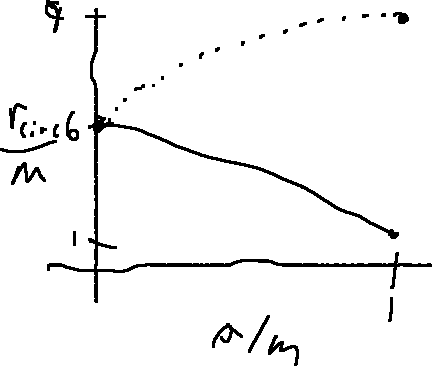
\includegraphics[width=12cm]{2-25-1.png}
	\caption*{The inner most stable radius for a circular orbit as a function of spin, the dotted lines are counter rotating}
\end{figure*}
For $a=M$ we see $e= \frac{1}{\sqrt{3}}$ $l = \frac{2M}{\sqrt{3}}$ and $r_\text{isco} = M$.
\subsection{Binding Energy}
The binding energy is the difference between the energy of a particle at rest at $\infty$ and the energy that the particle has moving in an orbit, as measured at infinity.

Since our rest mass energy is 1, we can say the binding energy per unit rest mass is $1-e$
\begin{figure*}[h]
	\centering
	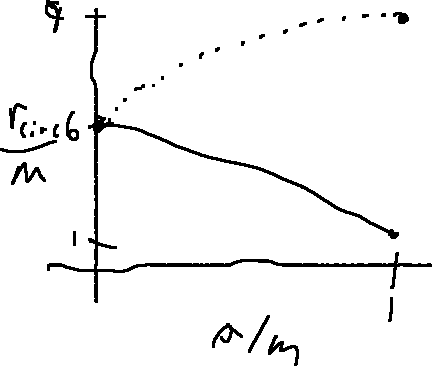
\includegraphics[width=12cm]{2-25-1.png}
	\caption*{Binding energy as a function of spin, the dotted line is counterrotating}
\end{figure*}
Clearly our corating ISCO is the ``most bound'' orbit, with this releasing $42\%$ of the rest mass energy of the particle when placed into this orbit.
\subsection{Ergosphere}
For the Schwartzchild geometry we can always remain a stationary observer as long as we are outside of the Schwarzchild radius. We want to consider what is needed to achieve this in the Kerr geometry (and whether or not it is even achievable).
To remain stationary we want:
\begin{align*}
	u^\alpha &= (u^t,0,0,0)
\end{align*}
And we know:
\begin{align*}
	-1 &= g_{tt} (u^t)^2 \\
	-1 &= -\left(1- \frac{2Mr}{\rho^2}\right) (u^t)^2 \\
\end{align*}
So this can only be satisfied when:
\begin{align*}
	r &> r_e & r_e &= M + \sqrt{M^2 - a\cos^2\theta}
\end{align*}
In order to avoid infall at a radius less that this new radius than we need to have our particle rotate along with the black hole.
